\documentclass[12pt,a4paper]{article}
\usepackage[utf8]{inputenc}
\usepackage[T1]{fontenc}
\usepackage{amsmath}
\usepackage{amsfonts}
\usepackage{amssymb}
\usepackage{graphicx}
\usepackage[left=2.54cm, right=2.54cm, top=2.54cm, bottom=2.54cm]{geometry}
\usepackage[hidelinks]{hyperref} %for reference automatically
\usepackage{fancyhdr}
\usepackage{subcaption}

\usepackage{tikz}
\usetikzlibrary{positioning}

\pagestyle{fancy} % for header and footer
\fancyhf{}
\fancyhead[LE,RO]{Prepared by: Phayuth}
\fancyhead[RE,LO]{Supervisor : Dr.Sarot Srang}
\fancyfoot[LE,RO]{Page \thepage}
\renewcommand{\headrulewidth}{2pt}
\renewcommand{\footrulewidth}{1pt} % for header and footer

% THIS IS THE XML CODE INCLUDE==============================================================
\usepackage{listings}
\usepackage{xcolor}
\definecolor{codegreen}{rgb}{0,0.6,0}
\definecolor{codegray}{rgb}{0.5,0.5,0.5}
\definecolor{codepurple}{rgb}{0.58,0,0.82}
\definecolor{backcolour}{rgb}{0.95,0.95,0.92}
\lstset{
	backgroundcolor=\color{backcolour},   
	commentstyle=\color{codegreen},
	keywordstyle=\color{magenta},
	numberstyle=\tiny\color{codegray},
	stringstyle=\color{codepurple},
	numbers=left,
	breaklines=true,
	tabsize=2,
	basicstyle=\ttfamily\footnotesize,
	literate={\ \ }{{\ }}1
}


\begin{document}
	\section*{\centering Foundation - Lesson 8 : Linear Approximation with Taylor Series}
	%	\begin{itemize}
		%		\item {\makebox[1cm]{\(x(t)\)\hfill} is Input of the system}
		%		\item {\makebox[1cm]{\(y(t)\)\hfill} is Output of the system}
		%		\item {\makebox[1cm]{\(h(t)\)\hfill} is the system}
		%	\end{itemize}
	
	%	\begin{equation}
		%		\boxed{
			%			H(s) = \frac{Y(s)}{X(s)}
			%		}
		%		\label{eq3}
		%	\end{equation}
	
	\section{What is a Linear System ?}
	Linear System is a system that comply to 2 rules.
	\begin{itemize}
		\item Superposition (Addition).
		\item Homogeneous (Multiplication). 
	\end{itemize}
	
	\begin{center}
		\textbf{Superposition}
	\end{center}
	
	Given that we have a function \(y = f(x)\).
	\begin{itemize}
		\item If we have a value \(x_1\) substitute to the function we get \(y_1\) : \(y_1 = f(x_1)\)
		\item If we have a value \(x_2\) substitute to the function we get \(y_1\) : \(y_2 = f(x_2)\).
		\item If we have a value \(x_1 + x_2\) substitute to the function we should get \(y_1+y_2\) : \(y_1+y_2 = f(x_1+x_2)\)
	\end{itemize}
	
	\begin{center}
		\textbf{Homogeneous}
	\end{center}
	
	Given that we have a function \(y = f(x)\).
	\begin{itemize}
		\item If we have a value \(\alpha x_1\) substitute to the function we get \(y_1\) : \(y_1 = f(\alpha x_1)\)
		\item If we have a value \(x_1\) substitute to the function then multiply by \(\alpha\) we should get \(y_1 = \alpha f(x_1)\)
	\end{itemize}
	
	\subsection{Example}
	
	\begin{itemize}
		\item Find out if the function is linear : \(y = x\)
	\end{itemize}
	\textbf{Superposition test:} \\
	\(y_1 = x_1\) \\
	\(y_2 = x_2\) \\
	Add both result together \(y_1 + y_2 = x_1 + x_2\) \\
	Substitute \(x_1 + x_2\) to the function we get \(y_1+y_2\). Thus, \(y_1+y_2=y_{12}\). TEST PASS.
	\textbf{Homogeneous test:} \\
	Substitute \(\alpha x\) we get \(y = \alpha x\) \\
	Substitute \(x\) and multiply by \(\alpha\) we get \(y = \alpha x\). Thus, \(\alpha x=\alpha x\). TEST PASS. \\
	Both test is passed and thus the system is linear.
	
	\begin{itemize}
		\item Find out if the function is linear : \(y = x^2\)
	\end{itemize}
	\textbf{Superposition test:} \\
	\(y_1 = x_1^2\) \\
	\(y_2 = x_2^2\) \\
	Add both result together \(y_1 + y_2 = x_1^2 + x_2^2\) \\
	Substitute \(x_1 + x_2\) to the function we get \((x_1+x_2)^2\). Thus, \(y_1+y_2!=y_{12}\). TEST FAIL. \\
	The test is failed and thus the system is nonlinear.
	
	\break
	
	
	\section{Linearization Process}
	One of the Linearization method is by using Tyler Expansion Series within an operational range for stability.
	\[
	y \approx y(x_0) + \left[\frac{dy}{dx}|_{x_0}\frac{(x-x_0)}{1!}\right] + \left[\frac{d^2y}{dx^2}|_{x_0}\frac{(x-x_0)^2}{2!}\right] + ... [Higher Order Term]
	\]
	Let take a look at the plot:
	
	\begin{figure}[h]
		\centering
		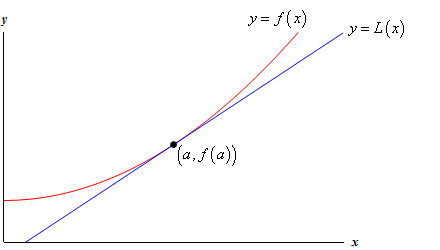
\includegraphics[width=0.7\linewidth]{src/fig1}
		\label{fig:Plot}
	\end{figure}
	
	\(y=L(x)\) is the linear approximation of \(y=f(x)\) and \(a = x_0\) is an equilibrium point. We can see that we want to pick an operational range where the function is stable because the \(y=L(x)\) is close to \(y=f(x)\). As we move a way from the operational range, the approximation is starting to diverge from the real solution.
	
	
	\subsection{Example}
	\begin{itemize}
		\item Linearize : \(y = x^2\)
	\end{itemize}
	We have:
	\[
	y \approx y(x_0) + \left[\frac{dy}{dx}|_{x_0}\frac{(x-x_0)}{1!}\right] + \left[\frac{d^2y}{dx^2}|_{x_0}\frac{(x-x_0)^2}{2!}\right] + ... [Higher Order Term]
	\]
	Only consider the first order term and eliminate HOT because in HOT the variable \(x\) is subject to power number that will make it nonlinear. We get:
	\[
	y \approx y(x_0) + \left[\frac{dy}{dx}|_{x_0}\frac{(x-x_0)}{1!}\right]
	\]
	We get:
	\[
	\frac{dy}{dx}|_{x_0} = \frac{d(x^2)}{dx}|_{x_0} = 2x|_{x_0} = 2x_0
	\]
	We get:
	\[
	\begin{split}
		y &\approx y(x_0) + \left[2x_0\frac{(x-x_0)}{1!}\right]\\
		y &\approx y(x_0) + \left[2x_0(x-x_0)\right]
	\end{split}
	\]
	\[
	\boxed{y \approx y(x_0) + 2x_0x-2x_0^2}
	\]
	Let pick an equilibrium point \(x_0=2\)
	\[
	\begin{split}
		y &= 2^2 + 2\times2x-2\times2^2 \\
		y &= 4+4x-8 \\
		y &= 4x-4
	\end{split}
	\]
	Now that we have a original function \(y=x^2\) and approximation function at \(x_0 = 2\) \(y=4x-4\). Let compare:
	\[
	\begin{split}
		x &= 2 \\
		=>y_{ori} &= 2^2 = 4 \\
		=>y_{lin} &= 4\times2 - 4 = 4
	\end{split}
	\]
	Both are equal to each other at equilibrium point.
	\[
	\begin{split}
		x &= 3 \\
		=>y_{ori} &= 3^2 = 9 \\
		=>y_{lin} &= 4\times3 - 4 = 8
	\end{split}
	\]
	A way from the equilibrium point, it starts to diverge.
	
	
\end{document}